\subsection{Winkelhistogramme (Janneke)}
\label{sec:winkelhistogramme}

Um eine Karte anhand von Laserscans aufbauen zu können müssen diese so ausgerichtet werden, dass gleiche Wände auf gleichen Wänden liegen. Der erste Schritt um dies zu erreichen ist die Rotation, die die Scans zueinander haben, zu berechnen. Dies ist möglich, indem man für die beiden Scans Winkelhistogramme erstellt.

Ein Winkelhistogramm stellt die Winkel, die es in einem Scan gibt, dar. Diese werden durch gerade Linien die der Scanner sieht und deren Winkel zum Roboter bestimmt. Obwohl der Roboter nur 180 Grad nach vorne sieht geht das Histogramm in diskreten Schritten von -180 bis +180 Grad.

Da wir zunächst in einer Simulation getestet haben, in der wir perfekte Laserscanwerte bekommen, verfolgen wir zunächst einen naiven Ansatz. Hierzu werden je 2 aufeinanderfolgende Scanpunkte betrachtet deren Winkel mit folgender Formel in Radiant berechnet wird: $$angle = atan2(scan[i][1] - scan[i+1][1], scan[i][0] - scan[i+1][0]) * 180 /PI;$$ In Abbildung~\ref{fig:Winkelberechnung} ist der Roboter und eine Wand die dieser mit seinem Laserscanner aufnimmt schematisch dargestellt. An dieser Darstellung wird gezeigt, wie die Formel zur Winkelberechnung zustande kommt.

\begin{figure}
	\centering
	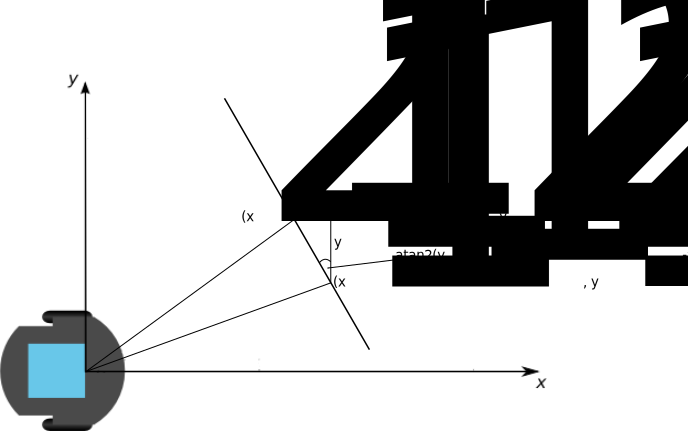
\includegraphics[width=11cm]{atan2}
	\caption{Winkelberechnung}
	\label{fig:Winkelberechnung}
\end{figure}

Der Winkel den man mit der oben ganannten Formel erhält wird in einen entsprechenden Bin im Histogramm umgerechnet, da dieses Diskret und nicht kontinuierlich ist. Dazu wurde folgende Formel verwendet, wobei BINCOUNT die Anzahl an Bins im Histogramm ist und damit die Auflösung bestimmt: $$\frac{(angle + 180) * BINCOUNT}{360}$$

Im Histogramm wird dann letztendlich festgehalten, wie oft ein bestimmter Bin (bzw. Winkelbereich) im Scan auftritt. Dadurch werden im Grunde die Wände bzw. geraden Linien die der Laserscanner erfasst dargestellt, da Scanpunkte die auf einer geraden Linie liegen relativ zum Roboter im gleichen Winkel stehen und somit in den gleichen Bin im Histogramm eingeortnet werden. So entsteht im Histogramm Peaks bei den Winkeln, die die Wände relativ zum Roboter haben.

\begin{figure}
	\centering
	\includegraphics[width=11cm]{winkelhistogramLaserOhneRauschen}
	\caption{Winkelhistogramm}
	\label{fig:Winkelhistogramm}
\end{figure}

In Abbildung~\ref{fig:Winkelhistogramm} ist das Winkelhistogramm welches wir mit diesem Ansatz erhalten haben zusammen mit dem Laserscan auf dem es berechnet wurde dargestellt.